\chapter{The CHERI Protection Model}
\label{chap:model}

This chapter describes the portable \textit{CHERI protection model}, its use
in software, and its impact on potential software vulnerabilities; concrete
mappings into computer architecture are left to later chapters.
We consider a number of topics from a more abstract, software-facing
perspectives: the principles underlying the model, our goals for capabilities,
hybridization with conventional architectural designs, implications for
operating-system and language support and compatibility, and concerns around
microarchitectural side channels.

There are many potential concrete mappings of this abstract software-facing
protection model into specific Instruction-Set Architectures (ISAs), but most
key aspects of the model can be shared across target architectures, including
the capability protection model, composition with virtual memory, and tagged
memory.
Whether used for memory protection or compartmentalization, CHERI's properties
hold with considerable uniformity across underlying architectural
implementations (e.g., regardless of capability size, whether capabilities are
stored in their own register file or as extensions to general-purpose integer
registers, etc.), and support common (and portable) programming
models and approaches.

We describe the cross-architecture aspects of CHERI in
Chapter~\ref{chap:architecture}.
Collectively, our instantiations of the CHERI protection model in the
32- and 64-bit RISC-V
(Chapter~\ref{chap:cheri-riscv}) and 64-bit ARMv8-A
(Morello~\cite{arm-morello}) ISAs
demonstrate the portability of the model despite diverse underlying
architectural implementations.

\section{Underlying Principles}

The design of CHERI is influenced by two broad underlying principles that are
as much philosophical as architectural, but are key to all aspects of the
design:

\begin{description}
\item[\textit{The principle of least privilege}] It should be possible to
  express and enforce a software design in which each program component can execute
  with only the privileges it requires to perform its function.
  This is expressed in terms of architectural privileges (e.g., by allowing
  restrictions to be imposed in terms of bounds, permissions, etc.,
  encapsulating a software-selected but hardware-defined set of rights) and at
  higher levels of abstraction in software (e.g., by allowing sealed
  capabilities to refer to encapsulated code and data incorporating both a
  software-selected and software-defined set of rights).
\psnote{the ``architectural privileges'' vs ``higher levels of
  abstraction'' conceptualization works a bit better here than on p.1,
  but it still seems iffy if I try to nail it down: the sealed caps
  are just as much in the ISA architecture as the first set}
  This principle has a long history in the research literature, and has been
  explored (with varying degrees of granularity) both in terms of the expression
  of reduced privilege (i.e., through isolation and compartmentalization) and
  the selection of those privileges (e.g., through hand separation, automated
  analysis, and so on).

\item[\textit{The principle of intentional use}]  When multiple rights
  are available to a program, the selection of rights used to authorize work
  on behalf of the program should be explicit, rather than implicit in the
  architecture or another layer of software abstraction.
  The effect of this principle is to avoid the accidental or unintended
  exercise of rights that could lead to a violation of the intended policy.
  It helps counter what are classically known as
  `confused deputy' problems, in which a program will unintentionally exercise
  a privilege that it holds legitimately, but on behalf of another program
  that does not (and should not) exercise that privilege~\cite{Hardy1988}.
  This principle, common to many capability systems but usually not explicitly
  stated, has been applied throughout the CHERI design, from architectural
  privileges (e.g., the requirement to explicitly identify capability
  registers used for load or store) through to the sealed capability mechanism
  that can be used to support object-capability models.
\end{description}

\noindent
These principles, which offer 
substantial mitigations against
 software vulnerabilities or malicious code, guide the integration
of a capability-system model with the general-purpose instruction set -- and
its exposure in the software model.
A more detailed exploration of the design principles embodied in and supported
by CHERI can be found in \textit{Fundamental Trustworthiness Principles in
CHERI}~\cite{neumann2017:cheri-principles}.

\section{CHERI Capabilities: Strong Protection for Pointers}

A key purpose of the CHERI protection model is to provide architectural
primitives to support strong protection for C and C++-language pointers.
Typically, language-level pointer types are implemented using architectural
integers in registers and in memory.
CHERI provides a new architectural data type, the \textit{capability}, which
software (such as a compiler) can use use instead when implementing pointers.
CHERI protections complement existing architectural protection mechanisms
such as virtual memory implemented by a Memory Management Unit (MMU) or
non-virtualized protection implemented by a Memory Protection Unit (MPU).
CHERI protections apply to the storage and manipulation of pointers, and also
accesses performed via pointers.
The rationale for this approach is two-fold:

\begin{enumerate}
\item A large number of vulnerabilities in Trusted Computing Bases (TCBs), and
  many of the application exploit techniques, arise out of bugs involving
  pointer manipulation, corruption, and use.
  These occur in several ways, with bugs such as those permitting attackers to
  coerce arbitrary integer values into dereferenced pointers, or leading to
  undesirable arithmetic manipulation of pointers or buffer bounds.
  These can have a broad variety of impacts -- including overwriting or leaking
  sensitive data or program metadata, injection of malicious code, and attacks
  on program control flow, which in turn allow attacker privilege escalation.

  Virtual memory fails to address these problems as (a) it is concerned with
  protecting data mapped at virtual addresses rather than being sensitive to
  the context in which a pointer is used to reference the address -- and hence
  fails to assist with misuse of pointers; and (b) it fails to provide
  adequate \textit{granularity}, being limited to page granularity -- or even
  more coarse-grained ``large pages'' as physical memory sizes grow.

\item Strong integrity protection, fine-grained bounds checking,
  encapsulation, and monotonicity for pointers can be used to construct
  efficient \textit{isolation} and \textit{controlled communication},
  foundations on which we can build scalable and programmer-friendly
  compartmentalization within address spaces.
  This facilitates deploying scalable application sandboxing with greater
  ubiquity, in turn mitigating a broad range of logical programming errors
  higher in the software stack, as well as resisting future undiscovered
  vulnerability classes and exploit techniques.

  Virtual memory also fails to address these problems, as (a) it scales
  poorly, paying a high performance penalty as the degree of
  compartmentalization grows; and (b) it offers poor programmability,
  as the medium for sharing is the virtual-memory page rather than the
  pointer-based programming model used for code and data sharing within
  processes.
\end{enumerate}

Consequently, \textit{CHERI capabilities} are designed to represent
language-level pointers with additional metadata to protect their integrity
and provenance, enforce bounds checks and permissions (and their
monotonicity), and hold additional fields supporting undereferenceable 
(i.e., sealed) software-defined
pointers suitable to implement higher-level protection models such as
separation and efficient compartmentalization.
Unlike virtual memory, whose functions are intended to be managed only by
low-level operating-system components such as kernels, hypervisors, and system
libraries, CHERI capabilities are also targeted more broadly at compiler and
language-runtime use, allowing program structure and dynamic memory allocation
to direct their use.
%We anticipate CHERI being used within operating-system kernels, and also in
%userspace libraries and applications, for the purposes of both memory
%protection and compartmentalization.

Significant attention has gone into providing strong compatibility with the C
and C++ programming languages, widely used in off-the-shelf TCBs such as
OS kernels and language runtimes, and also with conventional MMUs and
virtual-memory models -- which see wide use today and continue to operate on
CHERI-enabled systems.
This is possible by virtue of CHERI having a \textit{hybrid capability model}
that 
securely
composes a capability-system model with conventional architectural
features and programming-language pointer interpretation.
CHERI is designed to support incremental migration via selective recompilation
(e.g., transforming pointers into capabilities, as discussed below).
It provides several possible strategies for selectively deploying changes
into larger code bases -- constructively trading off source-code
compatibility, binary compatibility, performance, and protection.

Most source code can be recompiled to employ CHERI capabilities transparently
by virtue of existing pointer syntax and semantics, which the compiler can map
into capability use just as it currently maps that functionality into integer
address use -- while providing additional metadata to the architecture
allowing the implementation of stronger memory safety.
Code in which all pointers (and implied addresses) are implemented
solely using capabilities is referred to as \textit{pure-capability code}.
Capability use can also be driven selectively, albeit less transparently,
through annotation of C pointers and types to indicate that hybrid capability
code generation should be used when operating on those pointers -- referred to
as \textit{hybrid-capability code}.
It is also possible to imagine compilers making automatic policy-based
decisions about capability use on a case-by-case basis, based on trading off
compatibility, performance, and protection with only limited programmer
intervention.
It is further worth observing that, although the primary focus of CHERI has
been protecting pointers using capabilities, capabilities are a more
generalizable hardware data type that can be used to protect other types from
corruption and mis-manipulation.


\section{Architectural Capabilities}
\label{sec:architecturalcapabilities}

\psnote{Note to be associated with Figure~\ref{fig:fig-pointer-provenance}:
  Suggest we explain here what the boxes and arrows are, and how they
  illustrate those properties.  Are the horizontal bars all
  representations of the global (typically virtual) address space, with the
  coloured regions capabilities?  But then if the arrows are pointers
  (occurrences of capabilities), I don't understand why multiple
  arrows come from the same source?  Do Load/Store and Execute refer
  to the top-level bars, or are they just identifying the colours?}

\psnote{Also prompted by Figure~\ref{fig:fig-pointer-provenance}, but
  more generally: the
  text doesn't explain the terms used in its caption (provenance
  validity etc.), and they're a
  bit mysterious right now.  The Glossary does, and has a lot of other
  carefully considered good stuff besides, but it's 400 pages away and I guess few readers
  are going to spontaneously consult it.  We could (though I realise this might
  need an unachievable level of editing) in-line Glossary entries
  throughout the text where appropriate, while still (using latex
  macros to avoid forking) accumulating them in the Glossary at the end?}

\begin{figure}[t]
\centering
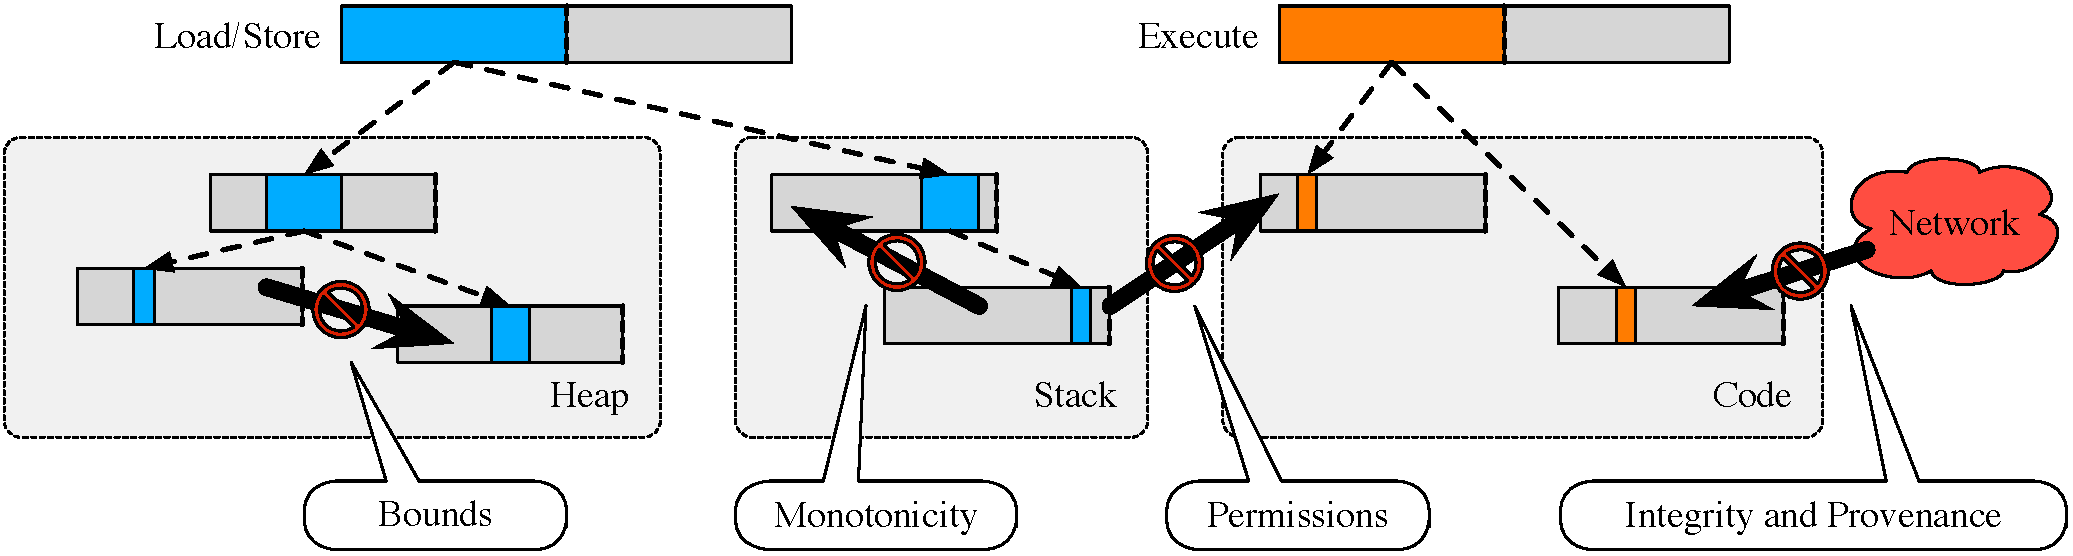
\includegraphics[width=\columnwidth]{fig-pointer-provenance.pdf}
\caption{CHERI enforces strict \textit{integrity}, \textit{provenance
validity}, \textit{monotonicity}, \textit{bounds}, \textit{permissions}, and
\textit{encapsulation} on pointers, mitigating common vulnerabilities and
exploit techniques.}
\label{fig:fig-pointer-provenance}
\end{figure}

In current systems, software typically implements pointers as integer values
stored in two architectural forms: in integer registers, and in memory.
\textit{Architectural capabilities} are a new architectural data type likewise
stored in register and memory, and containing an integer value that will most
frequently be interpreted as an address.
Capabilities also contain a number of other fields that contain additional
metadata associated with the address, such as bounds and permissions, as well
as a tag protecting their integrity.
Compilers, toolchains, and runtimes implementing pointers in terms of
architectural capabilities can imbue pointers with those protections, enforced
in hardware, subject to appropriately managing that metadata.
Capabilities are 2$\times$ (plus 1 bit) the size of the architecture's
natural address size, with the metadata compressed to fit in the additional
space.
On 32-bit architectures, capabilities are 64 bits ($+$1 tag bit), and on
64-bit architectures, capabilities are 128 bits ($+$1 tag bit).
In many senses, architectural capabilities used to implement pointers act like
the integers they replace, being loaded or stored, loaded or stored via,
jumped to, and so on.
The operating system, compiler, linker, and language runtimes are able to use
them to implement fine-grained memory safety for C and C++, as well as for
other purposes such as in-address-space software compartmentalization.

The majority of the capability is stored in a register or in
addressable memory, as is the case
for current integer pointers, with additional metadata stored adjacent to the
integer address it protects.
However, there is also a 1-bit tag that may be
inspected via the instruction set, but is not visible via byte-wise loads and
stores.
This tag is used to record whether the capability is valid; it is
preserved by legal capability operations but cleared by other architectural
operations on that memory.
%
Some of CHERI's protections are for pointers themselves (e.g., their integrity
and provenance validity), whereas others are for the pointee data or code
referenced by pointers (e.g., bounds and permissions).
CHERI's sealing feature protects both a pointer (via immutability) and the
pointee (via non-dereferenceability).

Extending architectures with capability registers and suitable memory storage
naturally aligns with many current architectural and microarchitectural design
choices, as well as software-facing considerations such as compiler code
generation, stack layout, operating-system behavior, and so on.
However, the generalized CHERI protection model can be mapped into
architectures in many different forms.
While implementation choices will affect a variety of factors in the
architecture and microarchitecture, the resulting protection model can be
considered \textit{portable} in that common protection properties and usage
patterns can be mapped into various architectural instantiations.
These topics are considered further in Chapter~\ref{chap:architecture}.

In the remainder of this section, we describe the high-level protection
properties and other functionality that capabilities grant to pointers and
the execution environment (see Figure~\ref{fig:fig-pointer-provenance}):

\begin{itemize}
\item Capability tags for pointer integrity and provenance
  (Section~\ref{sec:model-tags})
\item Capability bounds to limit the dereferenceable range of a pointer
  (Section~\ref{sec:model-bounds})
\item Capability permissions to limit the use of a pointer
  (Section~\ref{sec:model-permissions})
\item Capability monotonicity and guarded manipulation to prevent privilege
  escalation (Section~\ref{sec:model-monotonicity})
\item Capability sealing to implement software encapsulation
  (Section~\ref{sec:model-sealedcapabilities})
\item Capability object types to enable a software object-capability model
  (Section~\ref{sec:model-object-types})
\item Sealed capability invocation to implement non-monotonic domain
  transition (Section~\ref{sec:model-sealed-capability-invocation})
\item Capability control flow to limit pointer propagation
  (Section~\ref{sec:model-capability-control-flow})
\item Capability compression to reduce the in-memory overhead of pointer
  metadata (Section~\ref{sec:model-compression})
\item Hybridization with integer pointers
  (Section~\ref{sec:model-hybridization-integer-pointers})
\item Hybridization with MMU-based virtual memory
  (Section~\ref{sec:model-hybridization-virtual-addressing})
\item Hybridization with ring-based privilege
  (Section~\ref{sec:model-hybridization-architectural-privilege})
\item Failure modes and exception delivery
  (Section~\ref{sec:failuremodesandexceptions})
\item Capability revocation (Section~\ref{sec:model-capability-revocation})
\end{itemize}

\noindent
These features allow capabilities to be architectural primitives upon which
higher-level software protection and security models can be constructed (see
Section~\ref{sec:software-protection-using-cheri}).

\psnote{ perhaps the following subsections should be restructured to
 partition the description of what a capability comprises -- currently
 \ref{sec:model-tags}--\ref{sec:model-permissions} are basically doing
 that, though object types come later -- from the description of
 properties, which currently \ref{sec:model-monotonicity} onwards
 mostly are?   Or, if not, at least have a short bit here that briefly
 says what the data of a capability is.   Perhaps also with an
 \emph{illustrative} bit layout, emphasising that different arch
 instantiations will do things differently.  Could be a bit more
 specific about the permissions data, too.}

\subsection{Tags for Pointer Integrity and Provenance}
\label{sec:model-tags}

Each location that can hold a capability -- whether a capability register or a
capability-sized, capability-aligned word of memory -- has an associated 1-bit
tag that consistently and atomically tracks capability validity for the value
stored at that location:

\begin{description}
\item[Capability registers] each have a 1-bit tag tracking whether the
  in-register value is a valid capability.
  This bit will be set or cleared only as permitted by guarded manipulation.

\item[Capability-sized, capability-aligned words of memory] each have a 1-bit
  tag associated with the location, which is not directly addressable via data
  loads or stores: \textit{tagged memory}.
  Depending on the ISA variant, this may be at 64-bit or 128-bit granularity.
  The capability's address, as well as its other metadata such as
  bounds and permissions, are stored within the capability in addressable
  memory; these fields are protected by the corresponding unaddressable tag
  bit.
  If untagged memory exists in the system, the tags of capability values
  stored to those locations are discarded, and all loaded capability values
  will have the tag bit unset.
\end{description}

\noindent
Tags atomically follow capabilities into and out of capability registers when
their values are loaded from, or stored to, tagged memory.
Stores of other non-capability types -- e.g., of bytes or half words --
automatically and atomically clear the tag in the destination memory location.
This allows in-memory pointer corruption by data stores to be detected on next
attempted dereference -- for example, this prevents arbitrary data received
over the network from being directly dereferenced as a pointer.

The capability tag controls which operations can be performed using a
capability.
Attempting controlled operations on an untagged capability will cause a
precise exception.

Regardless of the value of the tag bit, capability register fields can be
accessed: they can be extracted and, subject to guarded manipulation,
modified.
Similarly, addressable portions of the capability can be read from memory
using ordinary data load and store instructions.
Capability values can also be loaded and stored via other valid capabilities
regardless of the validity of the loaded or stored capability.
An untagged capability value is simply data: allowing capability registers to
hold untagged values allows them to be used for capability-oblivious
operations.
For example, a region of memory can be copied via capability registers, including pointers within data structures, preserving the value of the
tag bit for each copied location.

However, other operations that \textit{dereference} or otherwise use a
capability require that the capability have its tag set -- i.e., be a
\textit{valid capability}.
Dereferencing refers to using the capability to load or store data or other
capabilities, or to fetch instructions.
This includes the implied dereference associated with the Default Data
Capability controlling legacy integer-relative loads and stores.
A valid tag is also required to use a capability to seal or unseal another
capability, to jump to that capability, to use it to set the architectural
compartment ID, or to call it for the purposes of domain transition.
Detailed information on which instructions require capabilities to have valid
tags, or operate on untagged capability values, may be found in the
instruction reference.

Valid capabilities can be constructed only by deriving them from existing
valid capabilities, which ensures \textit{pointer provenance}
(Figure~\ref{fig:fig-pointer-provenance}).
In almost all cases, a new capability value will be derived from a single
capability value -- e.g., as a result of reducing bounds or permissions.
In a few cases, a capability may derive from multiple other capability
values.
For example, a sealed capability is derived from both the authorizing sealing
capability and an original data capability.
Similarly, an explicitly unsealed capability is derived from both the sealed
capability and the capability that authorizes its unsealing.

Implementing C pointers as tagged capabilities allows them to be reliably
identified in the address space, which can help support techniques
such as garbage collection.

Our CHERI 
prototypes implement tagged memory using partitioned memory, with tags and
associated capability-sized units linked close to the memory controller, and
propagated by the cache hierarchy in order to provide strong atomicity with
the data it protects.
However, it is also possible to imagine implementations in which DRAM --
e.g., alongside ECC metadata -- or
non-volatile memory is extended to store tags with capability-sized units as
well.
We similarly assume that DMA will clear tags when writing to memory, although
it is possible to imagine future DMA implementations that are able to
propagate tags (e.g., to maintain tags on capabilities in descriptor rings).

\subsection{Bounds on Capabilities}
\label{sec:model-bounds}

Capabilities contain lower and upper bounds for the memory they authorize
access to.
While a capability's address may move out of bounds (and perhaps back in
again), attempts to dereference (e.g., via a load, store, or instruction
fetch) an out-of-bounds capability will throw a hardware exception.
This prevents exploitation of buffer overflows on global variables, the heap,
and the stack, as well as out-of-bounds execution.
Allowing addresses to sometimes be out-of-bounds with respect to their
bounds -- without faulting -- is important for de-facto C-language
compatibility.
In an ideal world, addresses could be arbitrarily out of bounds.
However, our
bounds-compression scheme places restrictions on this property, as bounds
compression depends on redundancy between the address and bounds, which is
reduced when addresses are substantially outside of their bounds (see
Section~\ref{compression} for details).

Bounds originate in allocation and linking events.
The operating system is able to place bounds on pointers to initial
address-space
allocations during process startup (e.g., via the initial register file, and
ELF auxiliary arguments in memory), and on an ongoing basis as new address-space
mappings are made available (e.g., via \ccode{mmap} system calls).
In practice, most bounds originate in the userspace language runtime or
compiler-generated
code, including the run-time linker for function pointers and global data,
the heap allocator for pointers to heap allocations, and generated code for
pointers taken to stack allocations.
 Programming languages may also offer explicit subsetting support to allow
software to impose its own expectations on suitable bounds for memory accesses
to complex objects (such as in-memory video streams) or in their own memory
allocators.

\subsection{Permissions on Capabilities}
\label{sec:model-permissions}
Capabilities additionally extend addresses with a permissions mask controlling how the
capability may be used.
For example, the run-time linker or compiler may set a capability's
permissions so that pointers to data cannot be reused for instruction fetch,
or so that pointers to code cannot be used to store data.
Further permissions control the ability to load and store capabilities
themselves, allowing the compiler to implement policies such as 
\textit{dereferenceable code and data pointers cannot be loaded from character
strings.}
Permissions can also be made accessible to higher-level aspects of the
run-time and programmer model, offering dynamic enforcement of concepts
similar to \ccode{const}.\footnote{The C-language \ccode{const} qualifier
conflates several orthogonal properties and thus can not be enforced
automatically.
Our language extensions include more constrained \ccode{\_\_input} and
\ccode{\_\_output} qualifiers.}
Languages may provide further facilities to allow programmer-directed
refinement of permissions -- for example, for use in Just-in-Time (JIT)
compilers.

Permissions changes, as with bounds setting, are often linked to allocation
events.
Permissions on capabilities for initial memory memory mappings can be
introduced by the kernel during process startup; further capabilities returned
for new mappings will also have their permissions restricted based on intended
use.
Executable capabilities representing function pointers and return addresses
will be refined by the run-time linker.
Read-only and read-write capabilities referring to data will be refined by the
run-time linker, heap allocator, and stack allocator.

Permissions also control access to the sealing facility used for encapsulation
(see Section~\ref{sec:model-sealedcapabilities}).
While sealing permission could be granted with all data and code capabilities,
best practice in privilege minimization suggests that a separate hierarchy
of sealing pointers should be maintained instead.
Returning independent sealing capabilities via a dedicated system-call
interface reduces opportunities for arbitrary code and data capabilities being
used improperly for this purpose.

\subsection{Capability Monotonicity via Guarded Manipulation}
\label{sec:model-monotonicity}

\textit{Capability monotonicity} is a property of the CHERI protection model
ensuring that new capabilities must be derived
from existing capabilities only via valid manipulations that may narrow (but
never broaden) rights ascribed to the original capability.
This property prevents broadening the bounds on pointers, increasing the
permissions on pointers, and so on, eliminating many manipulation attacks and
inappropriate pointer reuses.
Monotonicity also underlies effective isolation for software
compartmentalization by ensuring that delegated capabilities cannot be used to
reach other resources despite further manipulation.
CHERI enforces capability monotonicity via four mechanisms:

%across the vast majority of its
%instructions\psnote{what does ``vast majority'' mean here?  that it
%  doesn't enforce c.m. for some instructions, or that for some it
%  isn't by g.m., or what?}
%\knnote{The sealedness of a capability is not monotonic, but the
%  bounds and permissions of a capability are monotonic. To avoid
%  defining what ``vast majority'' means, \textit{capability
%    monotonicity} could also be replaced by \textit{capability bounds
%    monotonicity} and \textit{capability permission monotonicity}.}
%by 
%\psnote{think we can just delete this: ``virtue of \textit{guarded manipulation}: they cannot
%represent non-monotonic transformations.
%This is accomplished via''.  I don't see a need to introduce the
%``guarded manipulation'' concept, esp. if we're immediately
%eliminating it, and I don't know exactly what it means.}
% four mechanisms:

\begin{description}
\item[Limited expressivity] Some instructions are prevented, by design, from
  expressing an increase of rights due to the expression of their operands and
  implementation.
  For example, permissions on capabilities are modified using a bitwise `and'
  operation, and hence cannot express an increase in permissions.

\item[Stripping the tag in register write-back] Some instructions are able to
  represent non-monotonic operations, but attempts to use them
  non-monotonically will write back a capability with the tag bit
  cleared, preventing future dereference.
  Clearing the tag allows the failure to be discovered by an explicit
  software check, or on the next attempt to dereference.

\item[Exceptions on monotonicity violation] As an alternative to stripping
  the tag, attempts to use instructions non-monotonically could lead to an
  exception being delivered.
  We generally avoid this approach in favour of stripping the tag for the
  reasons discussed in Section~\ref{sec:rationale:tag-clear-vs-exception}.

\item[Stripping the tag in memory store] Tagged memory ensures that direct
  modification of capabilities stored in memory using data store instructions
  (whether non-monotonically or otherwise) will clear the tag on affected
  in-memory capabilities.
  This causes later attempts to dereference the capability to fail.
  This ensures that attempts to modify capabilities cannot bypass guarded
  manipulation.
\psnote{Add an analogous comment about debugging in this situation?
Are all such tag-clears indicative of bugs?  (not necessarily, given
strong updates, but perhaps).    Further to the
CHERI-as-perfect-sanitizer pitch, could we get eager detection here too,
by some combination of h/w and compiler support?}
\rwnote{No -- we frequently overwrite tagged values when storing a NULL,
  initialising memory, writing via another type in a union, doing a COW onto
  a page, etc.  There are surely cases where clearing the tag is a bug, but
  I suspect most cases are not.}

\end{description}

Selecting which enforcement mechanism to use will reflect the specific
operation being implemented, concerns about about ease of debugging, as well
as the context of the surrounding architecture. For example, in some
architectures, exceptions can be thrown on any instruction (e.g., MIPS), while
in others it is preferable for exceptions to be thrown only on memory
accesses (e.g., ARMv8-A).
As a result of these combined architectural features, guarded manipulation
implements \textit{non-bypassable capability monotonicity}.
\knnote{I don't know what ``non-bypassable'' means here: if the
  sentence would read ``\ldots implements capability monotonicity''
  would that already be enough? I also wonder whether this sentence
  should repeat that capabilities are not always monotonic.}

Monotonicity allows reasoning about the set of reachable rights for executing
code, as they are limited to the rights in any capability registers, and
inductively, the set of any rights reachable from those capabilities -- but no
other rights, which would require a violation of monotonicity.
\knnote{But CHERI does violate monotonicity. Perhaps it would help to
  introduce the exceptions to monotonicity first, and then discuss in
  this paragraph why these exceptions are not a problem for
  compartmentalization.}
Monotonicity is a key foundation for fine-grained compartmentalization, as it
prevents delegated rights from being used to gain access to other undelegated
areas of memory.
More broadly, monotonicity contributes to the implementation of the principle
of intentional use, in that capabilities not only cannot be used for
operations beyond those for which they are authorized, but also cannot
inadvertently be converted into capabilities describing more broad rights.

The two notable exceptions to strict monotonicity
\psnote{are these really exceptions to c.m. in the specific sense
  defined above, about the construction of new capabilities?   They
  have more to do with the lack of monotonicity of the permissions of
  the current hardware thread...}
 are invocation of sealed
capabilities (see Section~\ref{sec:model-sealed-capability-invocation}) and
exception delivery (see Section~\ref{sec:failuremodesandexceptions}).
\knnote{Is unsealing capabilities with \textit{CUnseal} an exception to monotonicity?}
Where non-monotonicity is present, control is transferred to code trusted to
utilize a gain in rights appropriately -- for example, a trusted
message-passing routine in the userspace runtime, or an OS-provided exception
handler.
This non-monotonicity is required to support protection-domain transition from
one domain holding a limited set of rights to destination domain that holds
rights unavailable to the originating domain -- and is therefore also
a requirement for fine-grained compartmentalization (see
Section~\ref{sec:model-isolation-controlled-communication-compartmentalization}).


\subsection{Capability Flags}
\label{sec:model-flags}
Capabilities include a flags field that can be manipulated freely.
Unlike the permissions field, it does not determine privilege, i.e., the state
of this field is orthogonal to capability monotonicity.
%
That is, these flags are intended to affect the \emph{semantics} of access,
rather than impose access control.
%
Currently, there are only architecture-specific interpretations for this
field: CHERI-RISC-V uses it to control opcode interpretation on instruction
fetch.
In the future, other non-security behavioral flags relating to capabilities may
be placed here, such
as to hint as to cache interactions for shared-memory rings, or to control
the behavior of operations such as capability equality testing.

\subsection{Sealed Capabilities}
\label{sec:model-sealedcapabilities}

Capability \textit{sealing} allows capabilities to be marked as
\textit{immutable} and \textit{non-deref\-erenceable}, causing the tag to be
cleared if attempts are made to modify them, and hardware exceptions to be
thrown if attempts are made to modify, dereference, or jump to them.
This enables capabilities to be used as unforgeable tokens of authority for
higher-level software constructs grounded in \textit{encapsulation}, while
still allowing them to fit within the pointer-centric framework offered by CHERI
capabilities.
There are two forms of capability sealing: pairs of capabilities sealed
using a common \textit{object type}, and stand-alone \textit{sealed entry
capabilities} (sentry capabilities).

Sealed pairs are primarily designed to support the linking of a pair of code
and data capabilities for use together during domain transition.
A jump-like instruction, \insnref{CInvoke}, allows the two sealed
capabilities to be atomically unsealed as control flow transfers to the code
pointed to by the code capability, if their object types match.
This can be used to implement controlled privilege escalation for the purposes
of domain transition.

Sealed entry capabilities simply seal a single code capability, which likewise
can be jumped to leading to an atomic unsealing and control-flow transfer.
This can also be used to implement domain transition with privilege
escalation, but to date has primarily been used to strengthen control-flow
robustness within a single protection domain by preventing the undesired
manipulation and use of code pointers.
Jump-and-link instructions acting on sealed entry capabilities also generate
a sealed return capability.

Sealed capabilities can also be used to support other operating-system or
language robustness features, such as representing other sorts of delegated
(non-hardware-defined) rights, or ensuring that pointers are dereferenced only
by suitable code (e.g., in support of language-level memory or type safety).

\rwnote{The next few subsections feel a bit redundant, and could be
  condensed.}

\subsection{Capability Object Types}
\label{sec:model-object-types}

Capabilities contain an additional piece of metadata, an \textit{object
type}\psnote{that sounds as if \emph{all} capabilities contain an
  object type...}%
\nwfnote{They do, at least implicitly!  \insnref{CGetType} returns
something, specifically $2^{64}-1$, for unsealed capabilities.  I've tried
to make the ISA speak in terms of \emph{encoding} the architectural
\cotype{} into the bit patterns of a capability, rather than being exactly
those bits, so that we can uniformly treat CC's separate \cotype{} field
and C-128's \csealed{} flag and shared \cotype{} bits.}%
, updated when a capability undergoes (un)sealing.
Object types allow multiple sealed capabilities to be indelibly (and
indivisibly) linked, so that the kernel or language runtime can avoid
expensive checks (e.g., via table lookups) to confirm that they are intended
to be used together.
%
\nwfnote{I am not sure I like ``indivisibly'' or maybe ``linked'' above; the indivisibility is
only up to ${\sim}/\cotype{}$, but it almost sounds like it's specifically a
pair of capabilities that are linked.  Perhaps ``associated''?}
%
For example, for object-oriented compartmentalization models,
pairs of sealed capabilities can represent
objects: one is the code capability for a class, and the other is a data
capability representing the data associated with a particular instance of an
object.

The object-type field is set when a capability is sealed based on a second
input capability authorizing use of the type space -- itself simply a
capability permission authorizing sealing within a range of values specified
by the capability's bounds.
A similar model authorizes \textit{unsealing}, which permits a sealed
capability to be restored to a mutable and dereferenceable state -- if a
suitable capability to have sealed it is held.

A similar model could be achieved without using an unsealing mechanism: a
suitably privileged component could inspect a sealed capability and rederive
its unsealed contents.
However, authorizing both sealing and unsealing based on type capabilities
allows the right to construct encapsulated pointers to be delegated, without
requiring recourse to a privileged software supervisor at the cost of
additional domain transitions -- or exercise of unnecessary privilege.

\subsection{Sealed Capability Invocation}
\label{sec:model-sealed-capability-invocation}

CHERI supports two forms of non-monotonicity\psnote{someone should
  revisit this phrasing after the glossary for monotonicity is sorted
  out: either that is only up to domain transitions, in which case
  these aren't non-..., or not, in which case these are}: jump-like capability invocation,
and exception handling (see Section~\ref{sec:failuremodesandexceptions}).
The \insnref{CInvoke} instruction accepts a pair of sealed
capability operands on which various checks are performed (for example, that
they are valid, sealed, and have matching object types).
If all tests are passed, then additional capabilities become available to the
executing CPU context by virtue of unsealing of the operand
registers.

The destination execution environment has well-defined and
reliable properties, such as a controlled target program-counter capability
and additional data capability that can be used to authorize domain
transition.
\insnref{CInvoke} behaves much like a conventional jump to register, permitting an
in-address-space domain switch without changing rings.

The newly executing code has the ability to further manipulate
execution state, and impose semantics such as call-return secure function
invocation or secure asynchronous message passing,
which will likely be followed by a privilege de-escalation as a target domain
is entered (see
Section~\ref{sec:model-isolation-controlled-communication-compartmentalization}).

\subsubsection{Object-Capability Policies in CHERI}

Consider an execution environment having access to several capabilities
sealed with the same \texttt{otype}.  The tests required by the
\insnref{CInvoke} mechanism describe a \emph{Cartesian product} of method
rights (indicated by the sealed code capability) and object rights (sealed data
capability) to this environment.  Regardless of how the environment
came to have these sealed capabilities, it is free to pair any sealed code
capability with any sealed data capability and have the \insnref{CInvoke}
tests pass.

Non-Cartesian and/or stateful policies can be encoded by
indirection, using memory to store additional data to be checked by the
invoked subsystem on entry.  The sealed data pointers given out by the
invoked subsystem now no longer directly reference objects; instead, they
reference ``data trampolines'' describing the pairing of object(s) \emph{and
remote agent(s)} with associated access rights information.  Attenuation of
access rights is no longer necessarily an ambiently available action and
requires either the explicit construction of membranes (i.e., proxy objects)
or active cooperation of the invoked subsystem (or an agent acting on its
behalf) to create new data trampoline(s).

\subsection{Capability Protection for Non-Pointer Types}

While the design of CHERI capabilities is primarily focused on the protection
of pointers, the pointer interpretation of capabilities depends entirely on
a capability's permissions mask.
If the mask authorizes load, store, and fetch instructions, then the
capability has a pointer interpretation.
\psnote{recent discussion in WG14/21 makes me sensitive to this:
  there's important code out there that relies on equality comparison
  of pointers to objects after lifetime-end of those objects, and the
  analogue of that in CHERI (with some temporal safety scheme) could
  be capabilities with tags or permissions cleared -- in which case
  they'd still have \emph{a} pointer interpretation, albeit a limited one}
Capabilities are not required to have those permissions set, however, allowing
capabilities to be used for other purposes -- for example, to protect other
critical data types from in-memory corruption (such as implementing UNIX file
descriptors or stack canaries), or to authorize access to system services
(such as authorizing use of specific system calls identified by the
capability).
Sealed capabilities and a set of software-defined permissions bits facilitate
these use cases by permitting non-architecture-defined capability
interpretations while retaining capability-based protections.

\subsection{Capability Flow Control}
\label{sec:model-capability-control-flow}

The CHERI capability model is designed to support the implementation of
language-level pointers: tagged memory allows capabilities to be stored in
memory, and in particular, embedded within software-managed data structures
such as objects or the stack.
CHERI is therefore particularly subject to a historic criticism of
capability-system models -- namely,
that capability propagation makes it difficult to track
down and revoke rights (or to garbage collect them).
To address this concern, CHERI has three mechanisms by which the flow of
capabilities can be constrained:

\begin{description}

\item[Capability PTE bits] extend the existing load and store
  permissions on page-table entries with new permissions to authorize loading and storing
  of capabilities.
  This allows the operating system to maintain pages from which tagged
  capabilities cannot be loaded (tags will be transparently stripped on load),
  and to which capabilities cannot be stored (a hardware exception will be
  thrown).
  This can be used, for example, to prevent tagged capabilities from being
  stored in memory-mapped file pages (as the underlying object might not
  support tag storage), or to create regions of shared memory through which
  capabilities cannot flow.

\item[Capability load and store permission bits] extend the load and store
  permissions on capabilities themselves, similarly allowing a capability to
  be used only for data access -- if suitably configured.
  This can be used to create regions of shared memory within an address
  space through which capabilities cannot flow.
  For example, it can 
prevent
  two separated compartments from
  delegating access to one another's memory regions, instead limiting
  communication to data traffic via the single shared region.
%%%% THE ORIGINAL SENTENCE WAS CONVOLUTED, ALLOWING SOMETHING NOT TO HAPPEN
%%%% DID NOT MAKE ANY SENSE.  ON THE OTHER HAND, I MAY HAVE GOTTEN THE FIX
%%%% BACKWARDS!

\item[Capability control-flow permissions] ``color'' capabilities to limit
  propagation of specific types of capabilities via other capabilities.
  This feature marks capabilities as \textit{global} or \textit{local} to
  indicate how they can be propagated.
  Global capabilities can be stored via any capability authorized for
  capability store.
  Local capabilities can be stored only via a capability specifically
  authorized as \textit{store local}.
  This can be used, for example, to prevent propagation of temporally
  sensitive stack memory between compartments, while still allowing
  garbage-collected heap memory references to be shared.

  This feature remains under development, as we hope to generalize it to
  further uses such as limiting the propagation of ephemeral DRAM references
  in persistent-memory systems.

\end{description}

The decision to strip tags on load, but throw an exception on
store\psnote{this might be rather opaque to readers -- did it refer to
  text that isn't there any more?  maybe expand to
explain?}, reflects
pragmatic software utilization goals: language runtimes and system libraries
often need to implement \textit{capability-oblivious memory copying}, as the
programmer may not wish to specify whether a region of memory must (or must
not) contain capabilities.
By stripping tags rather than throwing an exception on load, a
capability-oblivious memory copy is safe to use against arbitrary
addresses and source capabilities -- without risk of throwing an exception.
Software that wishes to copy only data from a source capability (excluding tag
bits due to a non-propagation goal) can simply remove the load-capability
permission from the source capability before beginning a memory copy.
%%%% THIS only SEEMS TO BE IN THE RIGHT PLACE: only specific data,
%%%% RATHER THAN data only from a source capability!!! 

On the other hand, it is often desirable to detect stripping of a capability on
store\psnote{this may also appear cryptic} via a hardware exception, to ease debugging.
For example, it is typically desirable to catch storing a tagged capability to
a file as early as possible in order to avoid debugging a later failed
dereference due to loss of a tag.
Similarly, storing a tagged capability to a virtual-memory page might be an
indicator to a garbage collector that it may now be necessary to scan that
page in search of capabilities.

This design point conserves PTE and permission bits; there is some argument
that completing the space (i.e., shifting to three or four bits
each\psnote{each what?}) would
offer functional improvements -- for example, the ability to avoid exceptions on
a capability-oblivious memory copy via a capability that does not authorize
capability store, or the ability to transparently strip tags on store to a
shared memory page.
However, we have not yet found these particular combinations valuable in our software experimentation, 

\subsection{Capability Compression}
\label{sec:model-compression}

\psnote{confusing contrast between ``in-memory representation'' and
  ``implementation'' -- I suspect better to position these as
  architectural alternates, rather than the latter as an
  ``implementation'' of the former}
\psnote{I suspect there needs to be some clarification across the
  whole document about whether ``128-bit'' refers to the old 128-bit
  scheme, or CHERI concentrate, or both? (and some particular version
  of concentrate?)}

Architecturally, capability fields are exposed via a set of accessor
instructions that get or set field values, such as the address, upper bound,
lower bound, and permissions.
The in-register and in-memory formats for capability contents may differ
substantially, permitting a more efficient representation using compressed
capability bounds.
CHERI utilizes a floating-point-like \textit{fat-pointer compression
technique} that relies on redundancy between the address, lower bound, and
upper bound.
The compressed representation exchanges stronger alignment requirements
(proportional to object size) for a more compact representation.

The CHERI Concentrate compression model (see Section~\ref{compression}) maintains monotonicity:
no ISA manipulation of a
capability can grant increased rights, and when unrepresentable cases are
generated
(e.g., a pointer substantially out of bounds, or a very unaligned object),
the pointer becomes un-dereferenceable.
Memory allocators already implement alignment requirements for heap and stack
allocations (word, pointer, page, and superpage alignments), and these
algorithms require only minor extension to ensure fully accurate bounds for
large memory allocations. Small allocations require no additional
alignment, where the definition of `small' depends on the compression format used and might be from 4 kiB to 1 MiB.
Relative to a 64-bit pointer, the 128-bit design reduces per-pointer memory
overhead (with a strong influence on cache footprint for some software
designs) by roughly two thirds, compared to, for example, a 256-bit
representation as found in earlier CHERI versions.

\subsection{Hybridization with Integer Pointers}
\label{sec:model-hybridization-integer-pointers}

Processors implementing CHERI capabilities also support existing programs
compiled to use conventional integer pointers, rather than capability
pointers, using two special capability registers:

\begin{description}
\item[Default Data Capability (DDC)] DDC indirects and controls legacy
  instructions that load and store relative to integer addresses rather than
  capabilities.

\item[Program Counter Capability (PCC)] PCC extends the conventional program
  counter with capability metadata, indirecting and controlling instruction
  fetches.
\end{description}

Programs compiled to use capabilities to represent pointers (whether
implicitly or via explicit program annotations) will not use the default data
capability, instead employing capability registers and capability-based
instructions for pointer operations and indirection.
The program-counter capability will be used regardless of the code model
employed, although capability-aware code generation will employ constrained
program-counter bounds and permissions to implement control-flow robustness
rather than using a single large code segment.
Support for legacy loads and stores can be disabled by installing a
sufficiently constrained (e.g., untagged) default data capability.

Different compilation modes and ABIs provide differing levels of compatibility
with existing code -- but include the ability to run entirely unmodified
non-CHERI binaries, to execute non-CHERI code in sandboxes within CHERI-aware
applications, and CHERI-aware code in sandboxes within CHERI-unaware
applications.

\subsection{Hybridization with Virtual Addressing}
\label{sec:model-hybridization-virtual-addressing}

\begin{figure}[t]
\centering
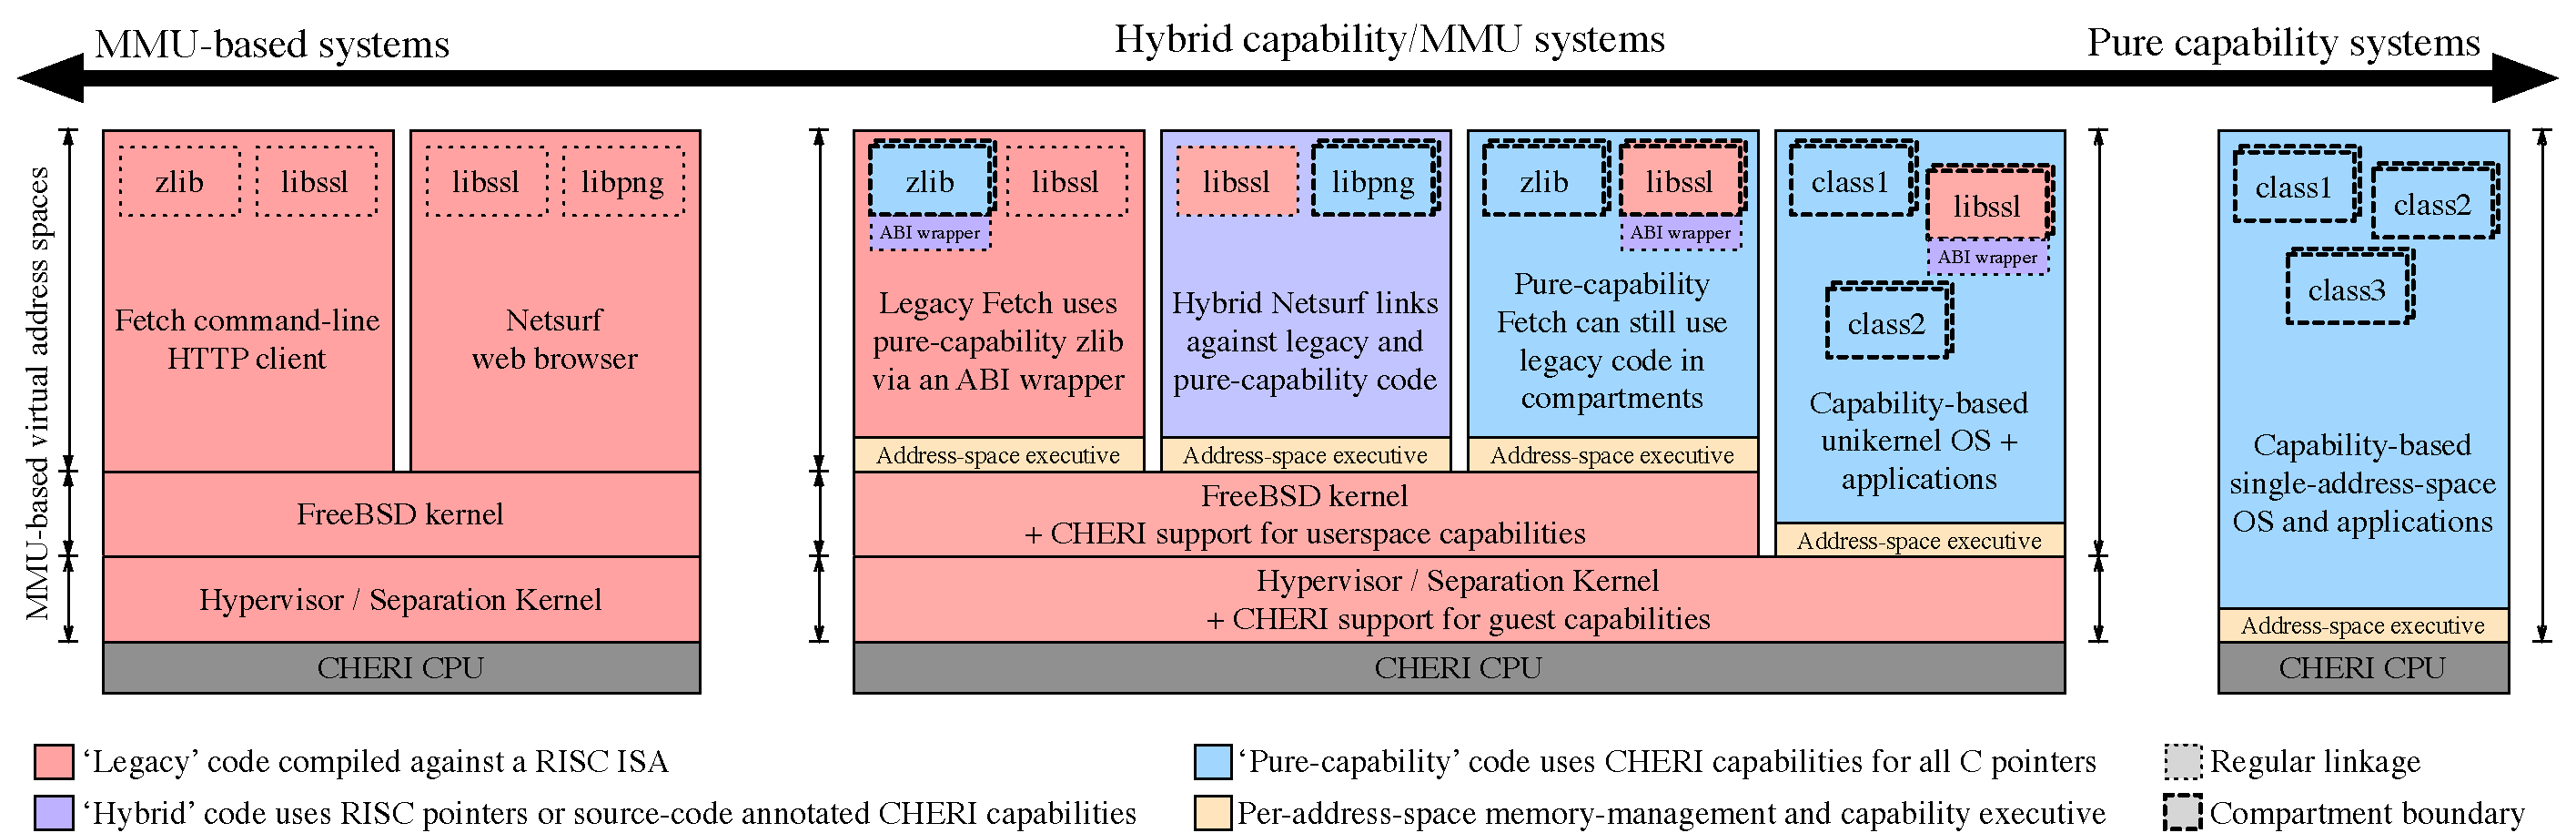
\includegraphics[width=\columnwidth]{fig-cheri-high-level.pdf}
\caption{CHERI supports a wide range of operational software models including:
unmodified MMU-based operating systems; hybrid operating systems
utilizing the MMU to support a process model and/or virtualization while
using CHERI within virtual address spaces; and pure single-address-space
CHERI-based operating systems.}
\label{fig:fig-os-models}
\end{figure}

The above features\psnote{which? just those in the preceding
  subsection, or all in this chapter?} compose naturally with, and complement, the Virtual-Memory (VM)
models commonly implemented using commodity Memory Management Units (MMUs) in
current OS designs (Figure~\ref{fig:fig-os-models}).
Capabilities are \textit{within} rather than \textit{between} address spaces;
they protect programmer references to data (pointers), and are intended to be
driven primarily by the compiler rather than by the operating system.
In-address-space compartmentalization complements process isolation by
providing fine-grained memory sharing and highly efficient domain switching
for use between compartments in the same application, rather than between
independent programs via the process model.
Operating-system kernels will also be able to use capabilities to improve the
safety of their access to user memory, as user pointers cannot be accidentally
used to reference kernel memory, or accidentally access memory outside of
user-provided buffers.
Finally, the operating system might choose to employ capabilities internally,
and even in its interactions with userspace, in referencing kernel data
structures and objects.

\subsection{Hybridization with Architectural Privilege}
\label{sec:model-hybridization-architectural-privilege}

Conventional architectures employ ring-based mechanisms to control use of
architectural privilege: only code executing in ``supervisor'' or ``kernel''
mode is permitted to access the virtual address space with supervisor rights,
but also to control the MMU, certain cache management operations,
interrupt-related features, system-call return, and so on.
The ring model prevents unprivileged code from manipulating the virtual
address space (and other processor features) in such a way as to bypass memory
protection and isolation configured by the operating system.
Contemporary instantiations may also permit virtualization of those features,
allowing unmodified operating systems to execute efficiently over microkernels
or hypervisors.
CHERI retains support for these models with one substantial modification: use
of privileged features within privileged rings, other than in accessing
virtual memory as the supervisor, depends on the program-counter capability
having a suitable hardware permission set.

This feature similarly allows code \emph{within} kernels, microkernels, and
hypervisors to be compartmentalized, preventing bypass of the capability model
within the kernel virtual address space through control of virtual memory
features.
The feature also allows vulnerability mitigation by allowing only explicit
use of privileged features: kernel code can be compiled and linked so that
most code executes with a program-counter capability that does not authorize
use of privilege, and only by jumping to selected program-counter capabilities
can that privilege be exercised, preventing accidental use.
Finally, this feature paves the way for process and object models in which the
capability model is used without recourse to rings.

\subsection{Failure Modes and Exceptions}
\label{sec:failuremodesandexceptions}

Bounds checks, permissions, monotonicity, and other properties of the CHERI
protection model inevitably introduce the possibility of new ISA-visible
failure modes when software violates rules imposed through capabilities
(whether due to accident or malicious intent).
We have selected to deliver failures as \textit{hardware exceptions}; for
example, on attempts to perform disallowed load and store operations, to
broaden bounds, and so on.
This allows the operating system (which in turn may delegate to the userspace
language runtime or application) the ability to catch and handle failures in
various ways -- such as by emulating disallowed accesses, converting to a
language-visible exception, or performing some diagnostic or mitigation
activity.

Different architectures express differing design philosophies for when
exceptions may be delivered, and there is flexibility in the CHERI model in
when exceptions might be delivered.
For example, while an attempt to broaden (rather than narrow) bounds could
generate an immediate exception, the operation could instead generate a
non-dereferenceable pointer as its output, in effect deferring an exception
until the time of an attempted load, store, or instruction fetch.
Both of these implementations ensure monotonicity by preventing derived
pointers from improperly allowing increased access following guarded
manipulation, and are consistent with the model.

Initially, in our prototyping, we selected to deliver exceptions as early as
possible when such events occur.
However, all current CHERI ISA instantiations defer exceptions to the use
of a capability's authority, instead clearing the tag on operations that
would otherwise violate monotonicity.

\pdrnote{The following two paragraphs perhaps belong in rationale?}
The early exception approach offers slightly improved debuggability
(by exposing the error earlier).
However, early exceptions limit compiler optimization as instructions that may
throw exceptions are restricted in how they can safely be reordered.
For example, this prevents a bounds restriction performed within a loop from
being hoisted outside the loop, unless that instruction is always executed.
If the loop is not always entered, this could turn a conditional execution
of a trapping instruction into an unconditional one.%
\footnote{This is not just a theoretical possibility -- we observed this
 happening in the FreeBSD kernel and had to modify the compiler to avoid
 hoisting any potentially-trapping CHERI instructions.}
In addition, code that manipulates untrusted capabilities is forced to branch
when the operation would be illegal, or risk being vulnerable to
denial-of-service attacks.
This may require it to recreate the hardware-performed checks in software.

With a deferred-exception approach, as well as avoiding these issues,
microarchitecture is simplified by reducing the set of instructions that can
throw exceptions.
While it is initially tempting to delay performing the required checks,
forwarding the common-case value and later flushing the pipeline if a check
fails, this leads to exploitable speculative side channel attacks.
As such, in either approach, microarchitecture must perform the checks
before forwarding the result.
Early exceptions can still be achieved if desired for debugging by
instrumenting potentially tag-clearing instructions with assertions about
the tag, either manually or in a compiler santitization pass.
The CHERI ISA design can ensure these checks are cheap, for example by
providing an instruction to throw an exception based on the tag.

\subsection{Capability Revocation, Garbage Collection, and Flow Control}
\label{sec:model-capability-revocation}

Revocation is a key design concern in capability systems, as revocation is
normally implemented via table indirection -- an approach in tension with the
CHERI design goal of avoiding table-based lookups or indirection on pointer
operations.
As described in Section~\ref{sec:model-capability-control-flow}, CHERI provides
explicit ISA-level features to constrain the flow of capabilities in order to
reduce the potential overhead in walking through memory to find outstanding
capabilities to resources (e.g., to implement garbage collection or sweeping
revocation).
There are also explicit features in the instruction-set architecture that
directly support the implementation of both pointer and object-capability
revocation:

\begin{description}
\item[MMU-based virtual-address revocation]
  As CHERI capabilities are evaluated prior to virtual addressing (i.e., they
  are pointers within address spaces), the MMU can be used not only to
  maintain virtual address spaces, but also to explicitly prevent the
  dereferencing of pointers to virtual address ranges -- regardless of the
  capability mechanism.
  Combined with a policy of either non-reuse of virtual address space (as
  distinct from non-reuse of physical address space), sweeping revocation, or
  garbage collection, this 
  allows all outstanding capabilities (and any further capabilities derived
  from them) to be revoked without the need to search for those capabilities
  in the register file or memory.
  This revocation is subject to the granularity and scalability limitations
  of MMUs: for example, it is not possible to revoke portions of the virtual
  address space smaller than one page.

  This low-level hardware mechanism must be combined with suitable software
  management of the virtual address space in order for it to be effective.
  For example, a policy of non-reuse of the virtual address space at
  allocation time will prevent stale capabilities from referring to a new
  allocation after an old one has been freed.
  A further policy of revoking MMU mappings for the region of virtual address
  space will prevent use of the freed memory as a communications channel from
  the point of free.
  Asynchronous and batched revocations will improve performance, subject to
  windows of opportunity in which use after free (but not use after
  re-allocation) might still be possible.
  It is also worth observing explicitly that non-reuse of the virtual address
  space in no way implies non-reuse of physical memory, as memory underlying
  revoked virtual addresses can be safely reused.
  An alternative to virtual address-space non-reuse is garbage collection, in
  which outstanding references to freed (and perhaps revoked) virtual address
  space are sought and explicitly invalidated.

  Use of the MMU for virtual address-space revocation is subject to a number
  of limits depending on the non-reuse and garbage-collection policies
  adopted.
  For example, if small, sub-page-size, tightly packed memory allocations
  are freed in a manner that leads to fragmentation (i.e., both allocated and
  freed memory within the same virtual page), then revocation will not be
  possible -- as it would prevent access to valid allocations (which could be
  emulated only at great expense).
  Similarly, fragmentation of the virtual address space may lead to greater
  overhead in the OS's virtual-memory subsystem, due to the need to maintain
  many individual small mappings, as well as the possibility of reduced
  opportunity to use superpages should revocations occur that are expressed
  in terms of smaller page sizes.

  However, overall, the MMU provides a non-bypassable means of preventing use
  of all outstanding capabilities to a portion of the virtual address space,
  permitting strong revocation to be used where appropriate.

\item[Accurate garbage collection]
  Traditional implementations of C are not amenable to accurate garbage
  collection because unions and types such as \ccode{intptr_t} allow a register
  or memory location to contain either an integer value or a pointer.
  CHERI-C does not have this limitation: The tag bit makes it possible to
  accurately identify all memory locations that contain data that can be
  interpreted as a pointer.
  Garbage collection is the logical dual of revocation: garbage collection
  extends the lifetime of objects as long as they have valid references, whereas
  revocation curtails the lifetime of references once the objects to which they
  refer are no longer valid.
  A simple stop-the-world mark-and-sweep collector for C can perform both tasks,
  scanning all reachable memory, invalidating all references to revoked objects, and recycling unreachable memory.

  More complex garbage collectors typically rely on read or write barriers
  (i.e., mechanisms for notifying the collector that a reference has been read or
  written).
  These are typically inserted by the compiler; however, in the context of revocation
  the compiler-generated code must be treated as untrusted.
  It may be possible to use the permission bits -- either in capabilities
  themselves or in page-table entries -- to introduce traps that can be used as
  barriers.

\item[Capability tags for sweeping revocation]
  In addition to supporting garbage collection, capability tags in registers
  and memory also allow the reliable identification of capabilities for the
  purposes of explicit revocation.
  Subject to safety in the presence of concurrency (e.g., by suspending
  software execution in the address space, or temporarily limiting
  access to portions of the address space), software can reliably
  sweep through registers and memory, clearing the tags (or otherwise
  replacing)
for
 capabilities that are to be revoked.
  This comes at potentially significant cost, which can be mitigated through
  use of the MMU -- e.g., to prevent capabilities from being used in certain
  pages intended only to store data, or to track where capabilities have been
  stored via a capability dirty bit in virtual-memory metadata.

\item[Revocation of sealed capabilities]
  When the interpretation of sealed capabilities is performed by a trustworthy
  software handler, there is the opportunity for that
  handler to implement revocation semantics explicitly.
  For example, the object invocation handler of a trusted userspace
  supervisor entered by \insnref{CInvoke}
  could interpret the
  address of a sealed capability as pointing to a table entry
  within its domain,
  rather than directly encapsulating a pointer to the target object's data.
  The address could be split into two parts: a table index, and a generation
  counter.
  The table entry could then itself contain a generation counter.
  Sealed object-capability references to the table entry would incorporate
  the value of the counter at the time of sealing, and the invocation handler
  would check the generation count, rejecting invocation on a mismatch.
  When object-capability revocation is desired, the table generation counter
  could be bumped, preventing any further use of outstanding references.
  This approach would be subject to limits on table-entry reuse and the size
  of the table; for example, a reasonable design might employ a 24-bit table
  index (permitting up to $2^{24}$ objects in the system at a time) and a
  40-bit generation counter.
  Use of the 24-bit object-type could further increase the number of objects
  permissible in the system concurrently.
  Many other similar schemes incorporating explicit checks for revocation
  based on software interposition employing counters, tables, etc., can be
  imagined.
\end{description}

CHERI includes several architectural features to facilitate techniques such
as garbage collection and sweeping revocation.
Tags allow capabilities to be accurately identified in both registers and
memory.
In addition, CHERI can limit the flow of capabilities via various mechanisms,
limiting the memory areas that must be swept for the two techniques: MMU
permissions controlling capability load and store via specific pages;
capability permissions controlling capability load and store via specific
capabilities; and the local-global feature that controls the propagation of
subsets of capabilities.
These primitives may be combined to support higher-level software policies
such as:

\begin{itemize}
\item ``capabilities may not be shared between address spaces''
\item ``local stack capabilities may be stored only to the local stack''
\item ``this shared-memory buffer can be used only for data sharing, not
  capability sharing''
\item ``capabilities can flow only one way through this shared buffer''
\item ``only the TCB can introduce capabilities to shared memory between
  compartments''
\item ``supervisor involvement is required to share sealed capabilities
  between compartments''
\item ``first store of a capability to any page will deliver an exception to
  the supervisor''
\end{itemize}

\noindent
As a result, garbage collection and sweeping revocation can rely on strong
invariants about capability propagation that limit the areas of memory that
must be swept for garbage collection or revocation.

\section{Software Protection and Security Using CHERI}
\label{sec:software-protection-using-cheri}

The remainder of the chapter explores these ideas\psnote{which?  just 2.3.16
\emph{Capability Revocation, Garbage Collection, and Flow Control}, or
everything in 2, or the section title?} in greater detail,
describing the high-level semantics
 offered
by the ISA and how they are mapped
into programmer-visible constructs such as C-language features.
The description in this chapter is intended to be agnostic to the specific
Instruction-Set Architecture (ISA) in which CHERI is implemented.  
In particular, it is important that programmers be able to rely on the
properties described in this chapter -- regardless of the ISA-level
implementation -- 
and that software abstractions built over these properties have 
consistent behavior that can be depended upon to mitigate vulnerabilities.

\subsection{Abstract Capabilities}

The CHERI architecture imposes tight constraints on capability manipulation and
use including provenance validity and monotonicity.
While these rules generally permit the execution of current C and C++ code
without significant modification, there are occasions on which the
programmer model of pointer properties (for example) may violate rules for
capabilities.
For example, the architecture maintains provenance validity of capabilities
from reset, permitting them to remain valid only if they are held in tagged
memory or registers.
In practice, operating systems may swap memory pages from DRAM to disk and
back, violating architectural provenance validity.
The OS kernel is able to maintain the appearance of provenance validity for
swapped pages by saving tags when swapping out, and re-deriving capabilities
from valid architectural capabilities when swapped back in -- maintaining the
\textit{abstract capabilities} that compiler-generated code works with.
Our ASPLOS 2019 paper on CheriABI explores this issue in
detail~\cite{davis2019:cheriabi}, covering topics such as context switching,
the C-language runtime, virtual-memory behavior, and debugging.

\subsection{C/C++ Language Support}

CHERI has been designed so that there are clean mappings from the C and C++
programming language into these protection properties.  Unlike
conventional virtual memory, the compiler (and not just the operating system)
is intended to play a significant role in managing these protections.
Protection is within address spaces, whether in a conventional user
process, or within the operating-system kernel itself in implementing its own
services or in accessing user memory:

\begin{description}
\item[Spatial safety]
CHERI protections are intended to directly protect the \textit{spatial safety}
of userspace types and data structures.  This protection includes
the integrity of pointers to code and
data, as well as implied code pointers in the form of return addresses and
vtable entries; bounds on heap and stack allocations; the  prevention
of executable data, and modification of executable code via permission.

\item[Temporal safety]
CHERI provides instruction-set foundations for higher-level \textit{temporal
safety} properties, such as non-reuse of heap allocations via garbage
collection and revocation, and compiler clearing of return addresses on the
stack.
In particular, the capability tags on registers and in memory allows pointers
to be reliably located and atomically replaced with a different value
(including an invalid capability).
Acceleration features allow capabilities to be located more efficiently than
simply sweeping all of physical memory.

\item[Software compartmentalization]
CHERI provides hardware foundations for highly efficient
\textit{software compartmentalization}, the fine-grained decomposition of
larger software packages into 
smaller isolated components that are 
granted access
only to the memory (and also software-defined) resources they actually require.

\item[Enforcing language-level properties]
CHERI's software-defined permission bits and sealing features can also be used
to enforce other language-level protection objectives (e.g., opacity of
pointers exposed outside of their originating modules) or to implement
hardware-assisted type checking for language-level objects (e.g., to more
robustly link C++ objects with their corresponding vtables).

\end{description}

\noindent
CHERI protections are implemented by a blend of 
functionality:

\begin{description}

\item[Compiler and linker] responsible for generating code that manipulates
  and dereferences code and data pointers, compile-time linkage, and 
  stack allocation.

\item[Language runtime] responsible for ensuring that program run-time
  linkage, memory allocation, and exceptions implement suitable policies in
  their refinement and distribution of capabilities to the application and its
  libraries.

\item[Operating-system kernel] responsible for interactions with conventional
  virtual memory, maintaining capability state across context switches,
  reporting protection failures via signals or exceptions, and implementing
  domain-transition features used with compartmentalization.

\item[Application program and libraries] responsible for distributing and
  using pointers, allocating and freeing memory, and employing higher-level
  capability-based protection features such as compartmentalization during
  software execution.

\end{description}

\subsubsection{Data-Pointer Protection}

Depending on 
the desired 
compilation mode, some or all data pointers will be implemented
using capabilities.
We anticipate that memory allocation (whether from the stack or heap, or via
kernel memory mapping) will return capabilities whose bounds and permissions
are suitable for the allocation, which will then be maintained for any derived
pointers, unless explicitly narrowed by software.
This will provide the following general classes of protections:

\begin{description}
\item[Pointer integrity protection] Overwriting a pointer in memory with data
  (e.g., received over a socket) will not be able to construct a
  dereferenceable pointer.

\item[Pointer provenance checking and monotonicity] Pointers must be derived
  from prior pointers via manipulations that cannot increase the range or
  permissions of the pointer.\psnote{TODO: check consistency with
    glossary for provenance after that's updated}

\item[Bounds checking] Pointers cannot be moved outside of their allocated
  range and then be dereferenced for load, store, or instruction fetch.

\item[Permissions checking] Pointers cannot be used for a purpose not granted
  by its permissions.
  In as much as the kernel, compiler, and run-time linker restrict
  permissions, this will (for example) prevent data pointers from being used
  for code execution.

\item[Bounds or permissions subsetting] Programmers can explicitly reduce the
  rights associated with a capability -- e.g., by further limiting its valid
  range, or by reducing permissions to perform operations such as store.
  This might be used to narrow ranges to specific elements in a data structure
  or array, such as a string within a larger structure.

\item[Flow control on pointers] Capability (and hence pointer) flow
  propagation can be limited using CHERI's capability flow-control
  mechanism, and used to enforce higher-level policies such as that
\textit{stack capabilities cannot be written to global data structures}, or
  that \textit{non-garbage-collectable capabilities cannot be passed across
  domain transitions}.
\end{description}

\subsubsection{Code-Pointer Protection}

Again with support of the compiler and linker, CHERI capabilities can be used
to implement control-flow robustness that prevents code pointers from being
corrupted or misused.
This can limit various forms of control-flow attacks, such as overwriting
of return addresses on the stack, as well as pointer re-use attacks such as
\textit{Return-Oriented Programming (ROP)} and \textit{Jump-Oriented
Programming (JOP)}.
Potential applications include:

\begin{description}
\item[Return-address protection] Capabilities can be used in place of pointers
  for on-stack return addresses, preventing their corruption.

\item[Function-pointer protection] Function pointers can also be implemented
  as capabilities, preventing corruption.

\item[Exception-state protection] On-stack exception state and signal
  frame information also contain pointers whose protection will limit
  malicious control-flow attacks.

\item[C++ vtable protection] A variety of control-flow attacks rely on either
  corrupting C++ vtables, or improper use of vtables, which can be detected
  and prevented using CHERI capabilities to implement both pointers to, and
  pointers in, vtables.
\end{description}

\subsection{Protecting Non-Pointer Types}

One key property of CHERI capabilities is that although they are designed to
represent pointers, they can also be used to protect other types -- whether
those visible directly to programmers through APIs or languages, or those used
only in lower-level aspects of the implementation to improve robustness.
A capability can be stripped of its hardware interpretation by masking all
hardware-defined permission bits (e.g., those authorizing load, store, and so
on).
A set of purely software-defined permission bits can be retrieved, masked, and
checked using suitable instructions.
Sealed capabilities further impose immutability on capability fields.
These non-pointer capabilities benefit from tag-based integrity and provenance
protections, monotonicity, etc.
There are many possible use cases, including:

\begin{itemize}
\item Using CHERI capabilities to represent hardware resources such as
  physical addresses, interrupt numbers, and so on, where software will
  provide implementation (e.g., allocation, mapping, masking), but 
where capabilities
  can be stored and delegated.

\item Using CHERI capabilities as canaries in address spaces: while stripping
  any hardware-defined interpretation, tagged capabilities can be used to
  detect undesired memory writes where bounds may not be suitable.

\item Using CHERI capabilities to represent language-level type information,
  where there is not a hardware interpretation, but unforgeable tokens are
  required -- for example, to authorize use of vtables by suitable C++
  objects.
\end{itemize}

\subsection{Protecting Physical Addresses}

A new capability type (distinguished using permissions, for example) could be
used to express and protect physical addresses.
The operating system would use these capabilities internally to control access
to physical addresses to IO memory, for example.
As most physical memory would be addressed using virtual memory mappings,
it would be natural to use physical capabilities as leaf node page table
entries (PTEs), reusing capability permissions as PTE permissions, though some
additional permissions would be necessary (e.g. dirty).

\paragraph{Synergy with linear capabilities and enclaves}
Linear physical capabilities could support low-overhead enclaves. 
If a physical capability could be linear, such that each instance is guaranteed
to be the unique reference to that physical memory, an enclave could be certain
that its virtual memory mapping is the only route to access that
physical page.
Additionally, it would be necessary to remove low-level page-table management
from the general operating system to ensure that the physical capability is not otherwise
dereferenced.

\paragraph{Synergy with sparse, contiguous page tables}
ASAP~\cite{margaritov2019prefetched} has proposed speculatively assuming that page
tables are contiguous, if sparse,
such that an address can directly index each level of
the page table to produce the probable address of its PTEs.  This allows all levels
to be queried in parallel, and will be likely to be correct if the operating system
succeeds in using the expected pages for the page table.
If the PTEs were capabilities of a unique type, it should be possible to
accurately distinguish a PTE from data.
With appropriate guarantees in page table layout (i.e. no overlapping contiguous
sparse page tables), the page walker can directly load the expected leaf entry
and know if it is a valid translation.
For practical contiguous page table sizes, it may be appropriate to use this
optimisation for the level before the leaf such that we have a fixed 2-level
page walk, at least in the common case.
We should note that this optimisation could be used apart from CHERI if physical
pages could be tagged to distinguish PTE pages from data pages.


\subsection{Isolation, Controlled Communication, and Compartmentalization}
\label{sec:model-isolation-controlled-communication-compartmentalization}

In \textit{software compartmentalization}, larger complex bodies of software
(such as operating-system kernels, language runtimes, web browsers, and office
suites) are decomposed into multiple components that run in isolation from one
another, having only selectively delegated rights to the broader application
and system, and limited further attack surfaces.
This allows the impact of exploited vulnerabilities or faults to be
constrained, subject to software being suitably structured -- i.e., that its
privileges and functionality have been suitable decomposed and safely
represented.
Software sandboxing is one example of compartmentalization, in which
particularly high-risk software is tightly isolated due to the risks it poses
-- for example, in rendering HTML\psnote{can be ambiguously read -- isolation of the
  HTML(!), or the rendering engine?} downloaded from a web site, or in processing
images attached to e-mail.
Compartmentalization is a more general technique, of which sandboxing is just
one design pattern, in which privileges are delimited and minimized to improve
software
robustness~\cite{Karger87,provos:preventingprivesc,Watson10,gudka15:soaap}.
Software compartmentalization is one of the few known techniques able to
mitigate future unknown classes of software vulnerability and exploitation, as
its protective properties do not depend on the specific vulnerability or
exploit class being used by an attacker.

Software compartmentalization is build on two primitives: \textit{software
isolation} and \textit{controlled communication}.
CHERI hybridizes two orthogonal mechanisms to construct isolation and
controlled communication: the conventional MMU (using multiple virtual address
spaces as occurs in widely used sandboxed process models), and CHERI's
in-address-space capability mechanism (by constructing
closures\psnote{not sure what that ``closures'' is supposed to mean -- closures in
  the PL sense? probably not.  boundaries?}  in the graph
of reachable capabilities).
These mechanisms can be combined to construct fine-grained software
compartmentalization within virtual address spaces, which may complement (or
even replace) a virtual-address-based process model.

To constrain software execution using CHERI, a more privileged software
runtime must arrange that only suitable capabilities are delegated to software
that must run in isolation.
For example, the runtime might grant software access to its own code, a stack,
global variables, and heap storage, but not to the private privileged state of
the runtime, nor to the internal state of other isolated software components.
This is accomplished by suitably initializing the thread register file of the
software (and hence CPU register file when it begins execution) to point into
an initial set of delegated code and allocation capabilities, and then
exercising discretion in storing capabilities into any further memory that it
can reach.
Capability nonforgeability, monotonicity, and provenance validity ensure
that new rights cannot be created by constrained software, and that existing
rights cannot be escalated.
As isolation refers not just to the initial state, but also the continuing
condition of software, discretion in delegating capabilities must be continued
throughout execution, in much the same way that software isolation using the
MMU depends not just on safe initial configuration, but safe continuing
configuration as code executes.

In order to achieve compartmentalization, and not simply isolation, CHERI's
selective non-monotonic\psnote{again: should check consistency of use
  of ``monotonicity'' following glossary fix} mechanisms can be used: exception handling, and
jump-based invocation.
If the software supervisor arranges that additional rights will be acquired by
the exception handler (using more privileged kernel code and data
capabilities), then the exception handler will be able to perform
non-monotonic transformations on the set of capabilities in the register file,
accessing memory (and other resources) unavailable to the isolated code.
Sealed capabilities allow encapsulated handles to resources to be delegated to
isolated code in such a manner that the sealed capabilities and resources they
describe can be protected from interference.
CHERI's jump-based invocation mechanism allows those resources to be unsealed
in a controlled manner, with control flow transferred to appropriate receiving
code in a way that protects both the caller and callee.
This source of non-monotonicity can also be used to implement domain
transition by having the caller discard rights prior to performing the jump,
and the callee acquire any necessary rights via unsealing of its capabilities.
It is essential to CHERI's design that exercise of non-monotonicity support
reliable transfer of control to code trusted with newly acquired rights.

Efficient controlled communication can persist across domain transitions
through the appropriate delegation of capabilities to shared memory, as well
as the delegation of sealed capabilities allowing selected domain switching.
CHERI's permissions allow uses of shared memory to be constrained in a
variety of ways.
The software configuring compartmentalization might choose to delegate
load-only or load-execute access to shared code or read-only data segments.
Other permissions constrain the propagation of capabilities; for example, the
software supervisor might allow communication only using data and not
capabilities via a communication ring between two mutually distrusting phases
in a processing pipeline.
Similarly, CHERI's local-global protections might be utilized to prevent
capabilities for non-garbage-collectable memory from being shared between
mutually distrusting components, while still allowing garbage-collectable heap
allocations to be delegated.

Collectively, these mechanisms allow a variety of software-defined
compartmentalization models to be constructed.
We have experimented with several, including
microkernel-based systems that utilize jump-based domain transition within
a single-address-space operating system, which model domain transition on
asynchronous or synchronous message passing.
Effective software compartmentalization relies not only on limiting access to
memory, but also a variety of other properties such as appropriate (perhaps
fair or prioritized) scheduling, resource allocation, and non-leakage of data
or rights via newly allocated or freshly reused memory, which are higher-level
properties that must be ensured by the software supervisor.
While many of these concerns exist in MMU-based software compartmentalization,
they can take on markedly different forms or implications.
For example, the zeroing of memory before reuse prevents the leakage of
rights, and not just data, in the capability model.
As with MMU-based isolation and compartmentalization, CHERI provides strong
architectural primitives, and is not intended to directly address
microarchitectural concerns such as cache side channels or information leakage
through branch predictors, performance counters, or other state.

Substantially different architectural underpinnings for capability-based,
rather than MMU-based, compartmentalization give it quite different practical
properties.
For example, two protection domains sharing access to a region of memory will
not experience increased page-table and TLB footprint by virtue of sharing a
virtual address space.
Similarly, the model for delegating shared memory is substantially different:
simple pointer delegation, rather than page-table construction, has far lower
overhead.
On the other hand, revoking access to shared memory via the capability model
requires either non-reuse of portions of the virtual address space, sweeping
capability revocation, or garbage collection (see
Section~\ref{sec:model-capability-revocation}).
We have found that the two approaches complement one another well: virtual
memory continues to provide a highly useful underpinning for conventional
coarse-grained virtual-machine and process models, whereas CHERI
compartmentalization works extremely well within applications as it caters to
rapid domain switching and large amounts of sharing between fine-grained and
tightly coupled components.

\subsection{Source-Code and Binary Compatibility}

CHERI supports Application Programming Interfaces (APIs) and
Application Binary Interfaces (ABIs) with compatibility properties intended
to facilitate incremental deployment of its features within current software
environments.
For example, an OS kernel can be extended to support CHERI capabilities in
selected userspace processes with only minor extensions to context switching
and process setup, allowing both conventional and CHERI-extended programs to
execute -- without implying that the kernel itself needs to be implemented
using capabilities.
Further, given suitable care with ABI design, CHERI-extended libraries can
exist within otherwise unmodified programs, allowing fine-grained memory
protection and compartmentalization to be deployed selectively to the most
trusted software (i.e., key system libraries) or least trustworthy (e.g.,
video CODECs), without disrupting the larger ecosystem.
CHERI has been tested with a large range of system software, and efficiently
supports a broad variety of C programming idioms poorly supported by the state
of the art in software memory protection.
It provides strong and reliable hardware-assisted protection in eliminating
common exploit paths that today can be mitigated only by using probabilistically
correct mechanisms (e.g., grounded in address-space randomization) that often
yield to determined attackers.

\subsection{Code Generation and ABIs}

Compilers, static and dynamic linkers, debuggers, and operating systems will
require extension to support CHERI capabilities.
We anticipate multiple conventions for code generation and binary interfaces,
including:

\begin{description}
\item[Conventional code generation] Unmodified operating systems, user
  programs, and user libraries will work without modification on CHERI
  processors.
  This code will not receive the benefits of CHERI memory protection --
  although it may execute encapsulated within sandboxes maintained by
  CHERI-aware code, and thus can participate in a larger compartmentalized
  application.
  It will also be able to call hybrid code.

\item[Hybrid code generation] Conventional code generation, calling
  conventions, and binary interfaces can be extended to support (relatively)
  transparent use of capabilities for selected pointers -- whether hand
  annotated (e.g., with a source-code annotation) or statically determined at
  compile time (e.g., return addresses pushed onto the stack).
  Hybrid code will generally interoperate with conventional code with
  relative ease -- although conventional code will be unable to directly
  dereference capability-based types.
  CHERI memory-protection benefits will be seen only for pointers implemented
  via capabilities -- which can be adapted incrementally based on tolerance
  for software and binary-interface modification.

\item[Pure-capability code generation] Software can also be compiled to use
  solely capability-based instructions for memory access, providing extremely
  strong memory protection.
  Direct calling in and out of pure-capability code from or to conventional
  code or hybrid code requires ABI wrappers, due to differing calling
  conventions.
  Extremely strong memory protection is experienced in the handling of both
  code and data pointers.

\item[Compartmentalized code] is accessed and can call out via
  object-capability invocation and return, rather than by more traditional
  function calls and returns.
  This allows strong isolation between mutually distrusting software
  components, and makes use of a new calling convention that ensures, among
  other properties, non-leakage of data and capabilities in unused argument
  and return-value registers.
  Compartmentalized code might be generated using any of the above models;
  although it will experience greatest efficiency when sharing data with other
  compartments if a capability-aware code model is used, as this will allow
  direct loading and storing from and to memory shared between compartments.
  Containment of compartmentalized components does not depend on the
  trustworthiness of the compiler used to generate code for those components.
\end{description}

Entire software systems need not utilize only one code-generation or
calling-convention model.  For example, a kernel compiled with conventional
code, and a small amount of CHERI-aware assembly, can host both hybrid
and pure-capability userspace programs.
A kernel compiled to use pure-capability or hybrid code generation could
similarly host userspace processes using only conventional code.
Within the kernel or user processes, some components might be compiled to be
capability-aware, while others use only conventional code.
Both capability-aware and conventional code can execute within
compartments, where they are sandboxed with limited rights in the broader
software system.
This flexibility is critical to CHERI's incremental adoption model, and
depends on CHERI's hybridization of the conventional MMU, OS models, and C
programming-language model with a capability-system model.

\subsection{Operating-System Support}

Operating systems may be modified in a number of forms to support CHERI,
depending on whether the goal is additional protection in userspace, in the
kernel itself, or some combination of both.
Typical kernel deployment patterns, some of which are orthogonal and may be
used in combination, might be:

\begin{description}
\item[Minimally modified kernel] The kernel enables CHERI support in the
  processor, initializes register state during context creation, and
  saves/restores capability state during context switches, with the goal of
  supporting use of capabilities in userspace.
  Virtual memory is extended to maintain tag 
integrity
  across swapping, and to prevent
  tags from being used with objects that cannot support them persistently
  -- such as memory-mapped files.
  Other features, such as signal delivery and debugging support require minor
  extensions to handle additional context.
  The kernel can be compiled with a capability-unaware compiler and limited
  use of CHERI-aware assembly.
  No additional protection is afforded to the kernel in this model; instead,
  the focus is on supporting fine-grained memory protection within user
  programs.

\item[Capability domain switching in userspace] Similar
  to the minimally modified kernel model, 
  only modest changes are made to the kernel itself.
  However, some additional extensions are made to the process model in order
  to support multiple mutually distrusting security domains within user
  processes.
  Access to system calls is limited to authorized userspace domains.

\item[Fine-grained capability protection in the kernel] In addition to
  capability context switching, the kernel is extended to support fine-grained
  memory protection throughout its design, replacing all kernel pointers with
  capabilities.
  This allows the kernel to benefit from pointer tagging, bounds checking, and
  permission checking, mitigating a broad range of pointer-based attacks such
  as buffer overflows and return-oriented programming.

\item[Capability domain switching in the kernel] Support for a
  capability-aware kernel is extended to include support for fine-grained,
  capability-based compartmentalization within the kernel itself.
  This in effect implements a microkernel-like model in which components of
the kernel, such as filesystems, network processing, etc., have only limited
  access to the overall kernel environment delegated using capabilities.
  This model protects against complex threats such as software supply-chain
  attacks against portions of the kernel source code or compiled kernel
  modules.

\item[Capability-aware system-call interface] Regardless of the kernel code
  generation model, it is possible to add a new system-call Application Binary
  Interface (ABI)
  that replaces conventional pointers with capabilities.
  This has dual benefits for both userspace and kernel safety.
  For userspace, the benefit is that system calls operating on its behalf will
  conform to memory-protection policies associated with capabilities passed to
  the kernel.
  For example, the \ccode{read} system call will not be able to overflow a
  buffer on the userspace stack as a result of an arithmetic error.
  For the kernel, referring to userspace memory only through capabilities
  prevents a variety of \textit{confused deputy problems} in which kernel bugs
  in validating userspace arguments could permit the kernel to access kernel
  memory when userspace access is intended, perhaps reading or overwriting
  security-critical data.
  The capability-aware ABI would affect a variety of user-kernel interactions
  beyond system calls, including ELF auxiliary arguments during program
  startup, signal handling, and so on, and resemble other
pointer-compatibility ABIs -- such as 32-bit compatibility for 64-bit kernels.
\end{description}

\noindent
These points in the design space revolve around hybrid use of CHERI
primitives, with a continued strong role for the MMU implementing a
conventional process model.
It is also possible to imagine operating systems created without taking this
view:

\begin{description}

\item[Pure-capability operating system] A clean-slate operating-system design
  might choose to minimize or eliminate MMU use in favor of using the CHERI
  capability model for all protection and separation.
  Such a design might reasonably be considered a \textit{single address-space
  system} in which capabilities are interpreted with respect to a single
  virtual address space (or the physical address space in MMU-free designs).
  All separation would be implemented in terms of the object-capability
  mechanism, and all memory sharing in terms of memory capability delegation.
  If the MMU is retained, it might be used simply for full-system
  virtualization (a task for which it is well suited), or also support
  mechanisms such as paging and revocation within the shared address space.
%\pgnnote{This alternative would be particularly relevant to dedicated
%  special-purpose CHERI processor systems, perhaps for input-output
%  microprocessors or Internet of Things device controllers.}

\end{description}

\section{Protection Against Microarchitectural Side-Channels}
\label{section:microarchitectural-sidechannels}

While CHERI has been designed as an architectural security mechanism -- i.e.,
one concerned with explicit access to memory contents or control of system
functions -- recent publication of highly effective attacks against
microarchitectural side channels has caused us to reconsider CHERI's potential
role~\cite{Kocher2018spectre}.
Several of these attacks (e.g., Spectre variants) rely on overly optimistic
speculative execution of paths that violate invariants embedded in the
executing code.
For example, code may contain explicit bounds checks, but by suitably training
a branch predictor, an attacker can cause the code to bypass those checks in
speculative execution, which then leaves behind a measurable result in the
instruction or data cache.
CHERI offers new opportunities to bound speculative execution such that it
observes security properties otherwise not explicitly available to the
microarchitecture.
Possible bounds on speculative execution grounded in CHERI features include:

\begin{itemize}
\item Enforcing capability tag checks in speculation, preventing code or data
  pointers without valid provenance from being used.
\item Enforcing capability bounds checks in speculation, preventing any
  out-of-bounds memory accesses for data load/store or instruction fetch.
\item Enforcing capability permission checks in speculation, preventing
  inappropriate loads or stores or instruction fetch.
\item Enforcing other capability protections, such as being sealed, to ensure
  encapsulation is implemented in speculation.
\item Limiting data-value speculation for capability values, or for values
  that will be combined with capabilities (e.g., integer values that are added
  to a capability offset to calculate a new capability).
\item Limiting speculation across protection-domain boundary transitions.
\end{itemize}

In addition, we have extended CHERI with new instructions to get and set a
software-defined \textit{compartment ID} (CID).
Unlike with conventional MMU-based virtual address spaces that have specific
address-space identifiers or page-table roots identifying protection domains,
CHERI protection domains are emergent from the dynamic delegation of
capabilities.
The CID might be used by microarchitectures to limit speculation of sharing
of microarchitectural state.
For example, branch-predictor entries may be tagged with a CID to prevent them
from being used with the wrong compartment.
This would necessarily need to be combined with an address-space identifier
(ASID), as addresses (and hence corresponding capabilities) may have different
interpretations in different address spaces.

As with other CHERI features, CID management is authorized using a capability,
allowing regions of CIDs to be delegated to domains or switchers for their
own selective use.
Where strong side-channel-free confidentiality is not required between a set
of domains, the CID may be left as-is.
Otherwise, a suitably authorized software domain switcher will be able to set
the CID to a new value.

Protective effects rely, of course, on appropriate implementation in the
microarchitecture.
Further notes on our thoughts on CHERI and microarchitectural side channels
may be found in our technical report, \textit{Capability Hardware Enhanced
RISC Instructions (CHERI): Notes on the Meltdown and Spectre Attacks}~\cite{UCAM-CL-TR-916}.
